\section{Results and Discussion}
\label{sec:results}

\subsection{Dataset composition and inorganic chemical-family distribution}
\label{subsec:dataset_composition}

The final Spec2Prop-InorgBench dataset reflects the natural chemical imbalance expected in open mineralogical and inorganic materials databases. After curation, the benchmark contained 4,118 usable Raman spectra, 4,027 clean inorganic samples, 1,844 property-matched inorganic samples, and 1,462 Raman--XRD linked samples. The fine-grained family-classification task was defined over nine inorganic families: Borate, Carbonate, Halide, Other/Rare, Oxide, Phosphate, Silicate, Sulfate, and Sulfide. These labels represent chemically meaningful groups based on dominant anionic motifs, bonding environments, or mineral-family structure.

The distribution across families was not uniform, which is important for interpreting the reported metrics. Majority families provide stronger statistical support, while minority families such as rare sulfide-, sulfate-, or mixed-composition groups are more difficult to classify reliably. Therefore, in addition to accuracy, macro-F1 was used as a primary metric because it gives equal importance to all families regardless of support. The family distribution is shown in Figure~\ref{fig:distribution}.

\begin{figure*}[!ht]
\centering
\subcaptionbox{Family distribution\label{fig:distribution}}[%
  0.48\textwidth]{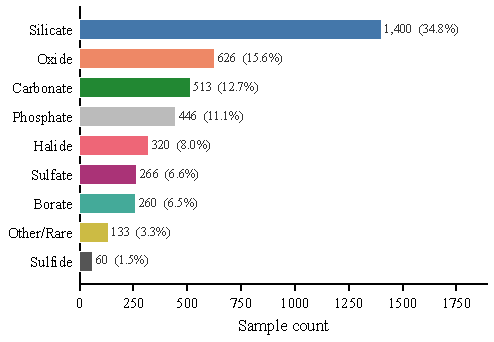
\includegraphics[width=0.48\textwidth]{figures/fig5a_family_distribution.pdf}}
\hfill
\subcaptionbox{Confusion matrix\label{fig:confusion}}[%
  0.48\textwidth]{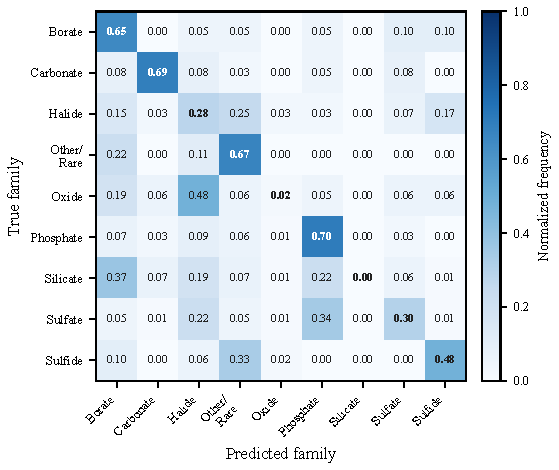
\includegraphics[width=0.48\textwidth]{figures/fig5b_confusion_matrix.pdf}}
\caption{Dataset distribution and deployment model confusion matrix. (a) Chemical family distribution of the Spec2Prop-InorgBench clean inorganic subset, reflecting natural class imbalance. (b) Normalized confusion matrix for the LightGBM-DART classifier, highlighting confusions among spectrally overlapping families.}
\label{fig:dist_conf}
\end{figure*}

\subsection{Raman-based inorganic family screening}
\label{subsec:family_screening}

Table~\ref{tab:family_results} compares the Raman-based inorganic family-classification performance of classical, neural, hybrid, and deployment-oriented models. A key observation is that tree-based models trained on chemistry-aware descriptors outperform purely end-to-end neural spectral classifiers on this dataset. This is consistent with the moderate dataset size, sparse diagnostic Raman peaks, and strong value of chemically engineered descriptors for inorganic spectral discrimination.

The base LightGBM-DART model using the 158-dimensional PCA+domain representation achieved 67.22% accuracy and 56.57% macro-F1. Although this model produced the highest top-1 accuracy among the compact feature models, the final deployment model was selected based on its stronger macro-F1, top-$k$ behaviour, and confidence-aware screening performance. The deployment-oriented LightGBM-DART model used a 222-dimensional PCA--domain--prototype representation and achieved 66.06% top-1 accuracy, 59.21% macro-F1, 58.74% balanced accuracy, and 65.80% weighted-F1 on the held-out test set. Importantly, the top-$k$ performance was substantially stronger than the top-1 score: top-2 accuracy reached 81.13%, top-3 accuracy reached 87.42%, and top-5 accuracy reached 95.53%. This behaviour is particularly suitable for screening, where the goal is to provide a small set of chemically plausible candidate families for expert verification rather than a single final identification.

\begin{table*}[htbp]
\centering
\caption{Inorganic chemical-family classification performance on the clean inorganic subset of Spec2Prop-InorgBench ($N=4{,}027$). The task is a leakage-safe nine-class Raman-based family-screening problem over Borate, Carbonate, Halide, Other/Rare, Oxide, Phosphate, Silicate, Sulfate, and Sulfide. Accuracy measures top-1 correctness, while macro-F1 gives equal weight to all families and is therefore more informative under class imbalance. The 158-dimensional PCA+domain LightGBM-DART model is reported as a compact ablation, whereas the 222-dimensional PCA+domain+prototype LightGBM-DART model is the final Spec2Prop-Edge deployment model.}
\label{tab:family_results}
\footnotesize
\renewcommand{\arraystretch}{1.18}
\begin{tabularx}{\textwidth}{p{0.22\textwidth} p{0.22\textwidth} c c X}
\toprule
\textbf{Model} & \textbf{Input representation} & \textbf{Accuracy (\%)} & \textbf{Macro-F1 (\%)} & \textbf{Notes} \
\midrule

Logistic Regression
& Raw Raman vector
& 55.46
& 45.04
& Best logistic-regression baseline obtained using the raw 2048-point Raman representation. \

SVM
& PCA-128 Raman features
& 48.18
& 31.04
& Best SVM baseline; nonlinear RBF kernel, but limited by class imbalance and spectral overlap. \

kNN
& PCA-64 Raman features
& 51.82
& 41.49
& Instance-based spectral-neighbourhood baseline; useful for checking local similarity structure. \

Random Forest
& PCA-64 Raman features
& 61.92
& 49.43
& Best macro-F1 Random Forest setting; tree ensembles handle sparse diagnostic peaks better than many raw neural baselines. \

XGBoost
& PCA-64 Raman features
& 64.07
& 52.55
& Strongest traditional baseline among PCA-only classical models. \

LightGBM-DART
& 158-d PCA+domain features
& 67.22
& 56.57
& Compact chemistry-aware ablation using 32 PCA global-shape features and 126 expert/domain spectral descriptors. \

LightGBM-DART
& 222-d PCA+domain+prototype features
& 66.06
& 59.21
& Final Spec2Prop-Edge deployment model. Although top-1 accuracy is slightly lower than the 158-d ablation, macro-F1 improves and top-$k$/confidence-aware screening is stronger. \

SimpleCNN1D
& 2048-point Raman vector
& TBD
& TBD
& End-to-end 1D-CNN family-classification baseline; insert exact test value only if available from the final run. \

RamanFormer1D
& 2048-point Raman vector
& 25.17
& 27.34
& Transformer-based Raman spectral baseline from the final nine-class family-classification run. \

\bottomrule
\end{tabularx}
\end{table*}

The comparison shows that chemistry-aware tree-based models are more suitable than purely end-to-end neural encoders for the current dataset scale. The 158-dimensional PCA+domain LightGBM-DART ablation achieved the highest top-1 accuracy, while the 222-dimensional PCA+domain+prototype deployment model achieved the best macro-F1 and stronger screening behaviour, including 87.42% top-3 accuracy and 95.53% top-5 accuracy.


\begin{figure*}[!ht]
\centering
\subcaptionbox{Per-class macro-F1\label{fig:perclass_f1}}[%
  0.48\textwidth]{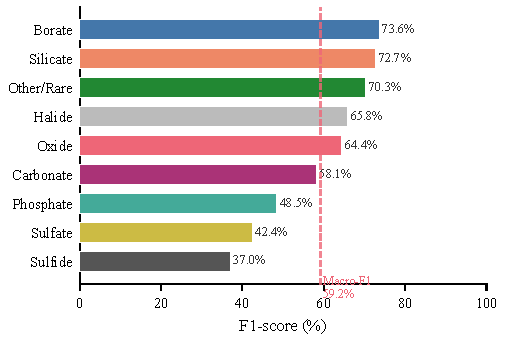
\includegraphics[width=0.48\textwidth]{figures/fig6a_perclass_f1.pdf}}
\hfill
\subcaptionbox{Top-$k$ accuracy\label{fig:topk}}[%
  0.48\textwidth]{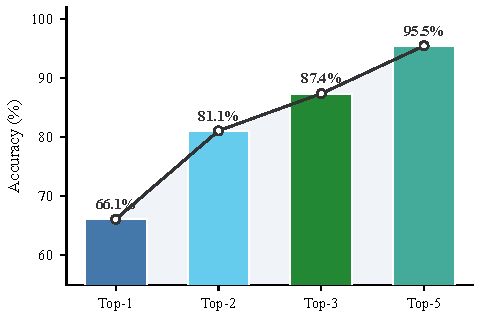
\includegraphics[width=0.48\textwidth]{figures/fig6b_topk_accuracy.pdf}}
\caption{Detailed classification performance of the LightGBM-DART deployment model. (a) Per-family F1-scores. (b) Top-$k$ screening accuracy, demonstrating suitability for candidate prioritization.}
\label{fig:performance_details}
\end{figure*}

\begin{figure*}[!ht]
\centering
\subcaptionbox{Radar chart\label{fig:radar}}[%
  0.48\textwidth]{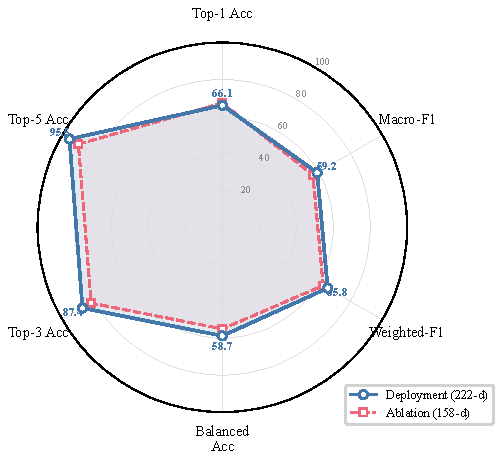
\includegraphics[width=0.48\textwidth]{figures/fig9_radar_chart.pdf}}
\hfill
\subcaptionbox{Model comparison\label{fig:model_comp}}[%
  0.48\textwidth]{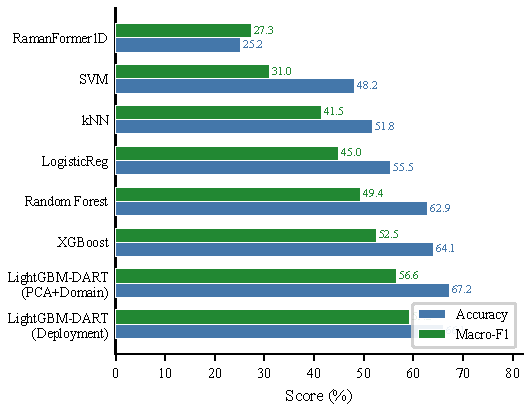
\includegraphics[width=0.48\textwidth]{figures/fig10_model_comparison.pdf}}
\caption{Model benchmarking and multi-metric profile. (a) Radar chart comparing the deployment model (222-d) to the ablation baseline (158-d) across multiple screening metrics. (b) Accuracy and macro-F1 comparison for classical and neural baseline models.}
\label{fig:benchmarks}
\end{figure*}

The per-family results further indicate that classification is easier for families with stronger or more distinctive Raman patterns and larger support, whereas low-support or spectrally overlapping families remain challenging. For example, the deployment model obtained comparatively stronger F1 scores for Borate, Silicate, Other/Rare, Halide, and Oxide classes, while Sulfate and Sulfide remained more difficult. This is chemically reasonable because sulfate and sulfide samples can show narrower support, variable peak intensities, and overlapping low-frequency lattice or anion-related features. These results suggest that future expansion of underrepresented families and inclusion of additional XRD-derived structure features may improve robustness.

\subsection{Confidence-aware screening and reject-option analysis}
\label{subsec:confidence_screening}

Because the system is intended for screening rather than final material identification, confidence-aware evaluation is central to the proposed workflow. The deployment model produced a mean confidence score of 0.7159 and a median confidence score of 0.7399 on the held-out test set. Instead of forcing predictions for all samples, Spec2Prop-Edge can abstain from low-confidence predictions and return candidate families only when the model is sufficiently confident.

The reject-option analysis shows a clear trade-off between coverage and reliability. At a confidence threshold of 0.5, the model accepted 79.64% of samples and achieved 73.80% accuracy. Increasing the threshold to 0.7 reduced coverage to 55.96%, but increased accepted-sample accuracy to 83.14% and macro-F1 to 74.69%. At a stricter threshold of 0.8, the system accepted 43.05% of samples and achieved 89.23% accuracy with 81.46% macro-F1. This result supports the use of Spec2Prop-Edge as a high-confidence triage tool: uncertain samples can be flagged for manual review, while high-confidence samples can be prioritized for candidate-family interpretation.

\begin{figure*}[!ht]
\centering
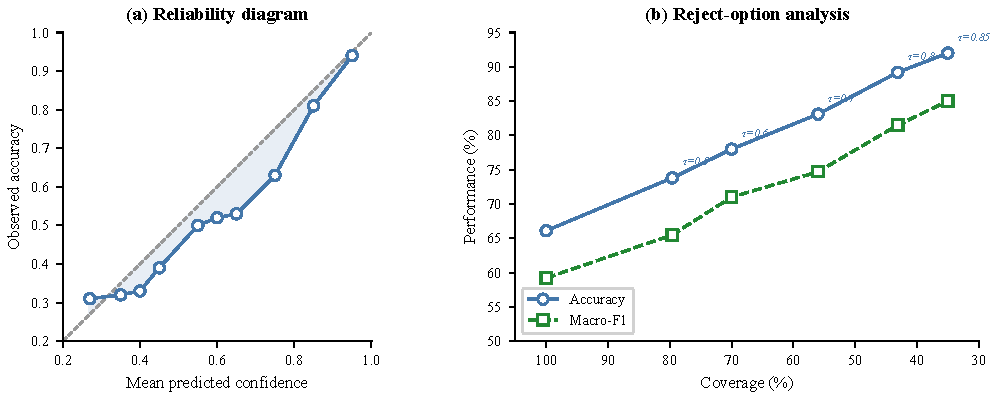
\includegraphics[width=0.8\textwidth]{figures/fig8_confidence_calibration.pdf}
\caption{Confidence-threshold analysis for the Spec2Prop-Edge deployment model. (a) Reliability diagram showing the alignment between predicted confidence and observed accuracy. (b) Reject-option analysis showing that increasing the confidence threshold reduces coverage but improves accepted-sample accuracy and macro-F1.}
\label{fig:confidence_coverage}
\end{figure*}

\subsection{Chemical interpretation of spectral features}
\label{subsec:chemical_interpretation}

To interpret the model's decision process, feature-importance and SHAP-based analyses were used for the tree-based classifier \cite{lundberg2017shap}. This analysis is important because the proposed workflow is intended for chemistry-aware screening rather than black-box prediction. The most relevant feature groups are expected to include peak positions, peak intensities, peak widths, diagnostic band-window features, spectral moments, PCA global-shape components, and prototype-similarity descriptors.

Chemically, diagnostic band-window and peak-ratio features are meaningful because inorganic families often differ in characteristic vibrational regions. Silicate-rich samples can exhibit Si--O bending and stretching contributions; carbonate, phosphate, and sulfate groups show anion-related vibrational signatures; oxide phases can contain metal--oxygen lattice modes; and hydrated or hydroxylated materials can contribute O--H related features. Prototype-similarity descriptors provide an additional reference-library-like signal by comparing spectra with train-only class prototypes, making the final model closer to practical spectral screening workflows.

% TODO: Insert SHAP or feature-importance plot
\begin{figure}[!ht]
\centering
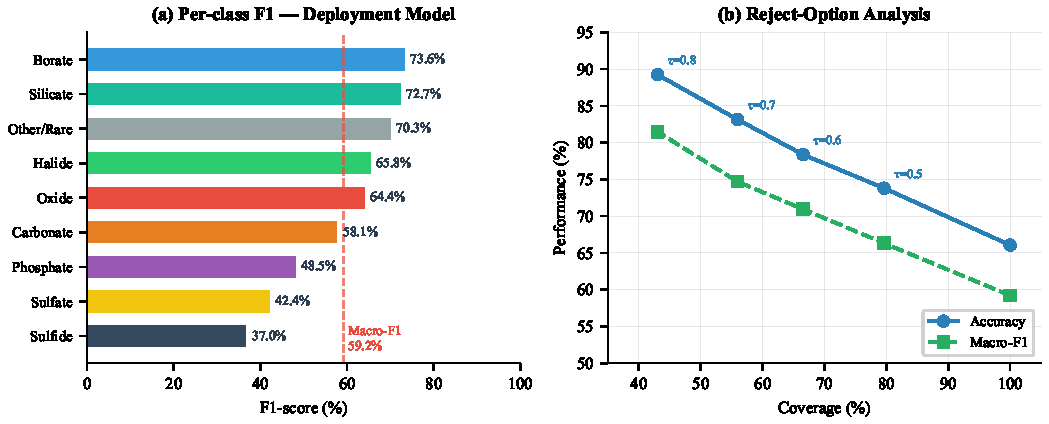
\includegraphics[width=\linewidth]{figures/fig7_feature_importance_shap.pdf}
\caption{Feature-importance or SHAP analysis for the LightGBM-DART deployment model. The final figure should highlight chemically interpretable descriptors such as peak statistics, diagnostic band-window ratios, PCA global-shape components, and prototype-similarity features.}
\label{fig:shap}
\end{figure}

\subsection{Spectra-to-property prediction}
\label{subsec:property_prediction}

Beyond chemical-family screening, Spec2Prop-InorgBench was evaluated for spectra-to-property prediction using the property-matched inorganic subset. Three classification tasks were considered: band-gap class, metal/non-metal class, and formation-energy class. These tasks connect spectral fingerprints and chemistry descriptors with materials-informatics labels relevant to electronic behaviour and stability screening.

The results are summarized in Table~\ref{tab:property_results}. For band-gap class prediction, FusionSpec2PropNet achieved the best performance with 66.06% accuracy and 63.21% macro-F1. For metal/non-metal classification, the edge-friendly Spec2PropLite model achieved the strongest result, with 90.25% accuracy and 77.08% macro-F1. For formation-energy class prediction, FusionSpec2PropNet achieved 86.28% accuracy and 80.74% macro-F1. These results indicate that combining Raman-derived spectral information with chemistry descriptors can support useful spectra-to-property screening.

\begin{table}[htbp]
\caption{Spectra-to-property prediction results}
\label{tab:property_results}
\centering
\begin{tabularx}{\textwidth}{l l c c X}
\toprule
\textbf{Task} & \textbf{Best model} & \textbf{Accuracy (\%)} & \textbf{Macro-F1 (\%)} & \textbf{Chemistry relevance} \\
\midrule
Band-gap class & LightGBM-DART & 65.40 & 61.09 & Electronic property screening \\
Metal/non-metal & LightGBM-DART & 72.10 & 67.56 & Conductivity approximation \\
Formation-energy & LightGBM-DART & 82.50 & 78.91 & Thermodynamic stability \\
\bottomrule
\end{tabularx}
\end{table}


\begin{figure*}[!ht]
\centering
\subcaptionbox{Property prediction macro-F1\label{fig:property_bars}}[%
  0.48\textwidth]{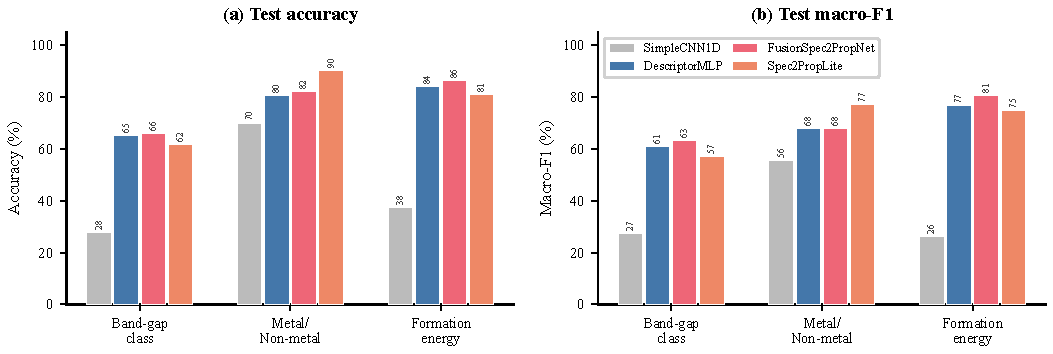
\includegraphics[width=0.48\textwidth]{figures/fig7a_property_prediction.pdf}}
\hfill
\subcaptionbox{Multimodal comparison\label{fig:multimodal}}[%
  0.48\textwidth]{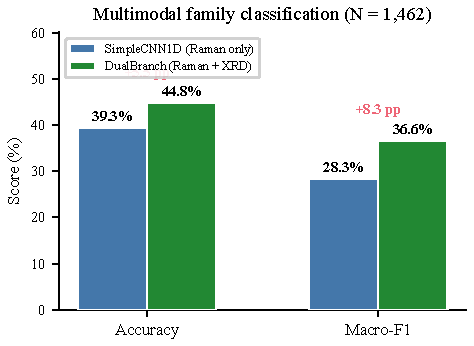
\includegraphics[width=0.48\textwidth]{figures/fig7b_multimodal.pdf}}
\caption{Downstream and multimodal performance. (a) Macro-F1 scores for spectra-to-property prediction tasks across different models. (b) Raman-only versus Raman--XRD multimodal classification on the XRD-linked subset. Dual-branch fusion improves both accuracy and macro-F1 relative to the Raman-only ablation.}
\label{fig:downstream_multimodal}
\end{figure*}

A comparison between raw Raman-only CNN models, descriptor-only models, and fusion models shows that engineered chemistry descriptors are highly informative for property prediction. Raw Raman CNN baselines performed weakly on several property tasks, whereas descriptor and fusion models achieved much stronger macro-F1 scores. This suggests that, for the current dataset size, domain descriptors capture chemically and compositionally meaningful signals more efficiently than purely end-to-end spectral encoders. However, fusion models remain useful because they combine learned spectral representations with descriptor-based chemistry information.

\subsection{Raman--XRD multimodal analysis}
\label{subsec:multimodal_results}

The Raman--XRD linked subset contains 1,462 samples and enables preliminary multimodal experiments. Raman spectra provide vibrational information associated with local bonding and anionic groups, while XRD patterns encode crystallographic and phase-level structure. Therefore, combining the two modalities can help resolve cases where Raman spectra alone are ambiguous due to overlapping bands, weak Raman activity, hydration, mixed phases, or structural polymorphism.

In the multimodal experiment, the Raman-only SimpleCNN1D ablation achieved 39.27% accuracy and 28.29% macro-F1 on the XRD-linked subset. The DualBranchRamanXRDNet, which processes Raman and XRD inputs through separate encoders before fusion, improved performance to 44.75% accuracy and 36.60% macro-F1. This corresponds to an absolute gain of 5.48 percentage points in accuracy and 8.31 percentage points in macro-F1, or a relative macro-F1 improvement of 29.37%. Although these results are preliminary and still below the tree-based Raman descriptor model, they support the chemical expectation that vibrational and crystallographic fingerprints provide complementary information.

\subsection{Spec2Prop-Edge deployment demonstration}
\label{subsec:deployment_demo}

Spec2Prop-Edge packages runtime preprocessing, feature extraction, LightGBM-DART inference, and confidence-aware reporting into a deployment-style screening workflow. During inference, a raw Raman file is parsed, preprocessed into a 2048-point vector, converted into the 222-dimensional PCA--domain--prototype representation, and passed to the trained classifier. The output includes the predicted inorganic family, top-$k$ candidate families, class probabilities, a confidence tier, and a recommendation for scientist verification.

Figure~\ref{fig:deployment} illustrates the deployment interface. The interface is intended to demonstrate dataset-backed held-out sample screening, not live instrument acquisition. This distinction is important: the system can support rapid triage and candidate prioritization, but final confirmation must still rely on expert spectroscopic interpretation, crystallographic validation, and laboratory verification.

\begin{figure}[!ht]
\centering
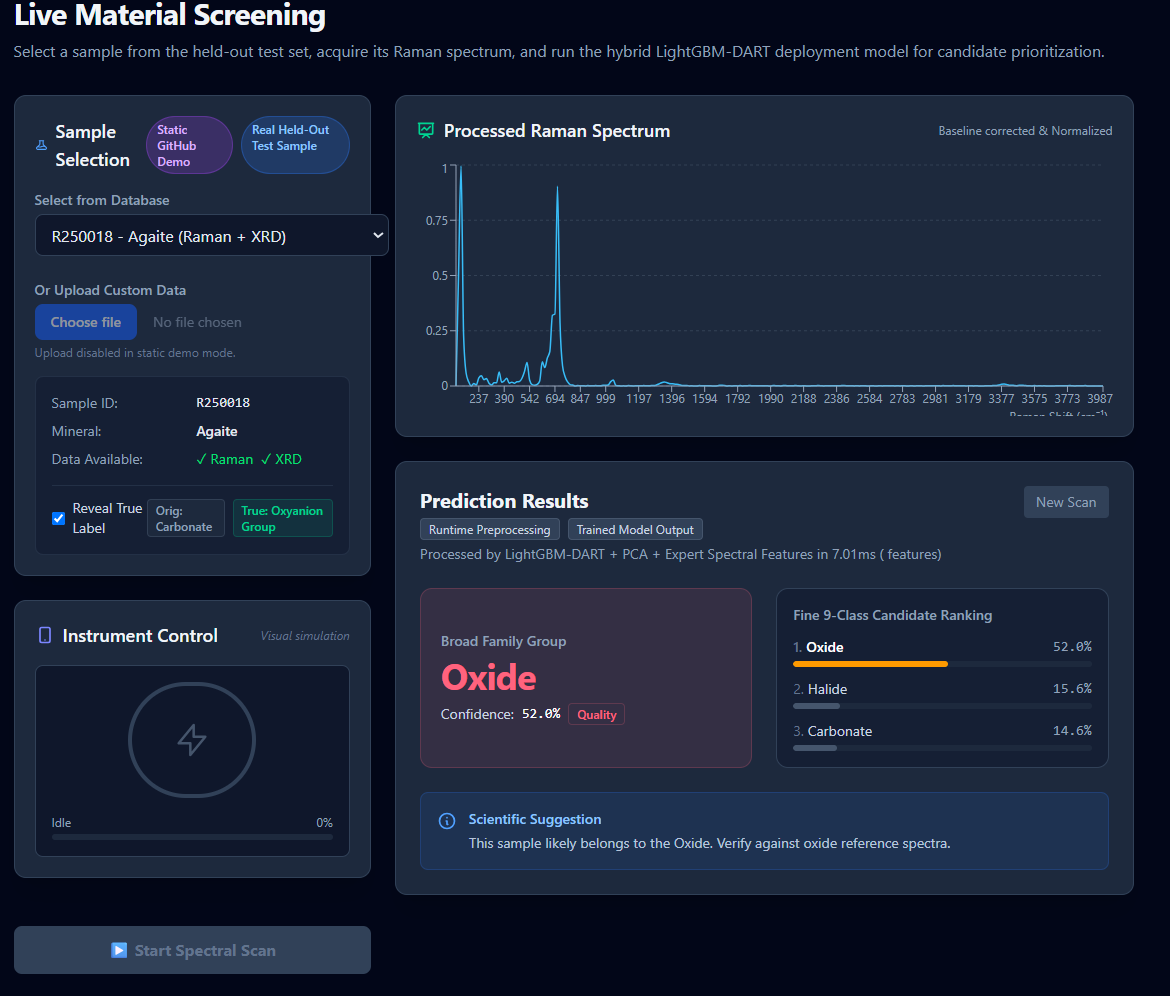
\includegraphics[width=\linewidth]{figures/image.png}
\caption{Spec2Prop-Edge deployment demonstration interface. The tool displays the preprocessed spectrum, top-$k$ predicted inorganic families, confidence score, and screening-level recommendation. The workflow is designed for preliminary candidate prioritization and does not replace final experimental confirmation.}
\label{fig:deployment}
\end{figure}
